\documentclass[crop,tikz,convert=pdf2svg]{standalone}
\usepackage{tikz}

\begin{document}
    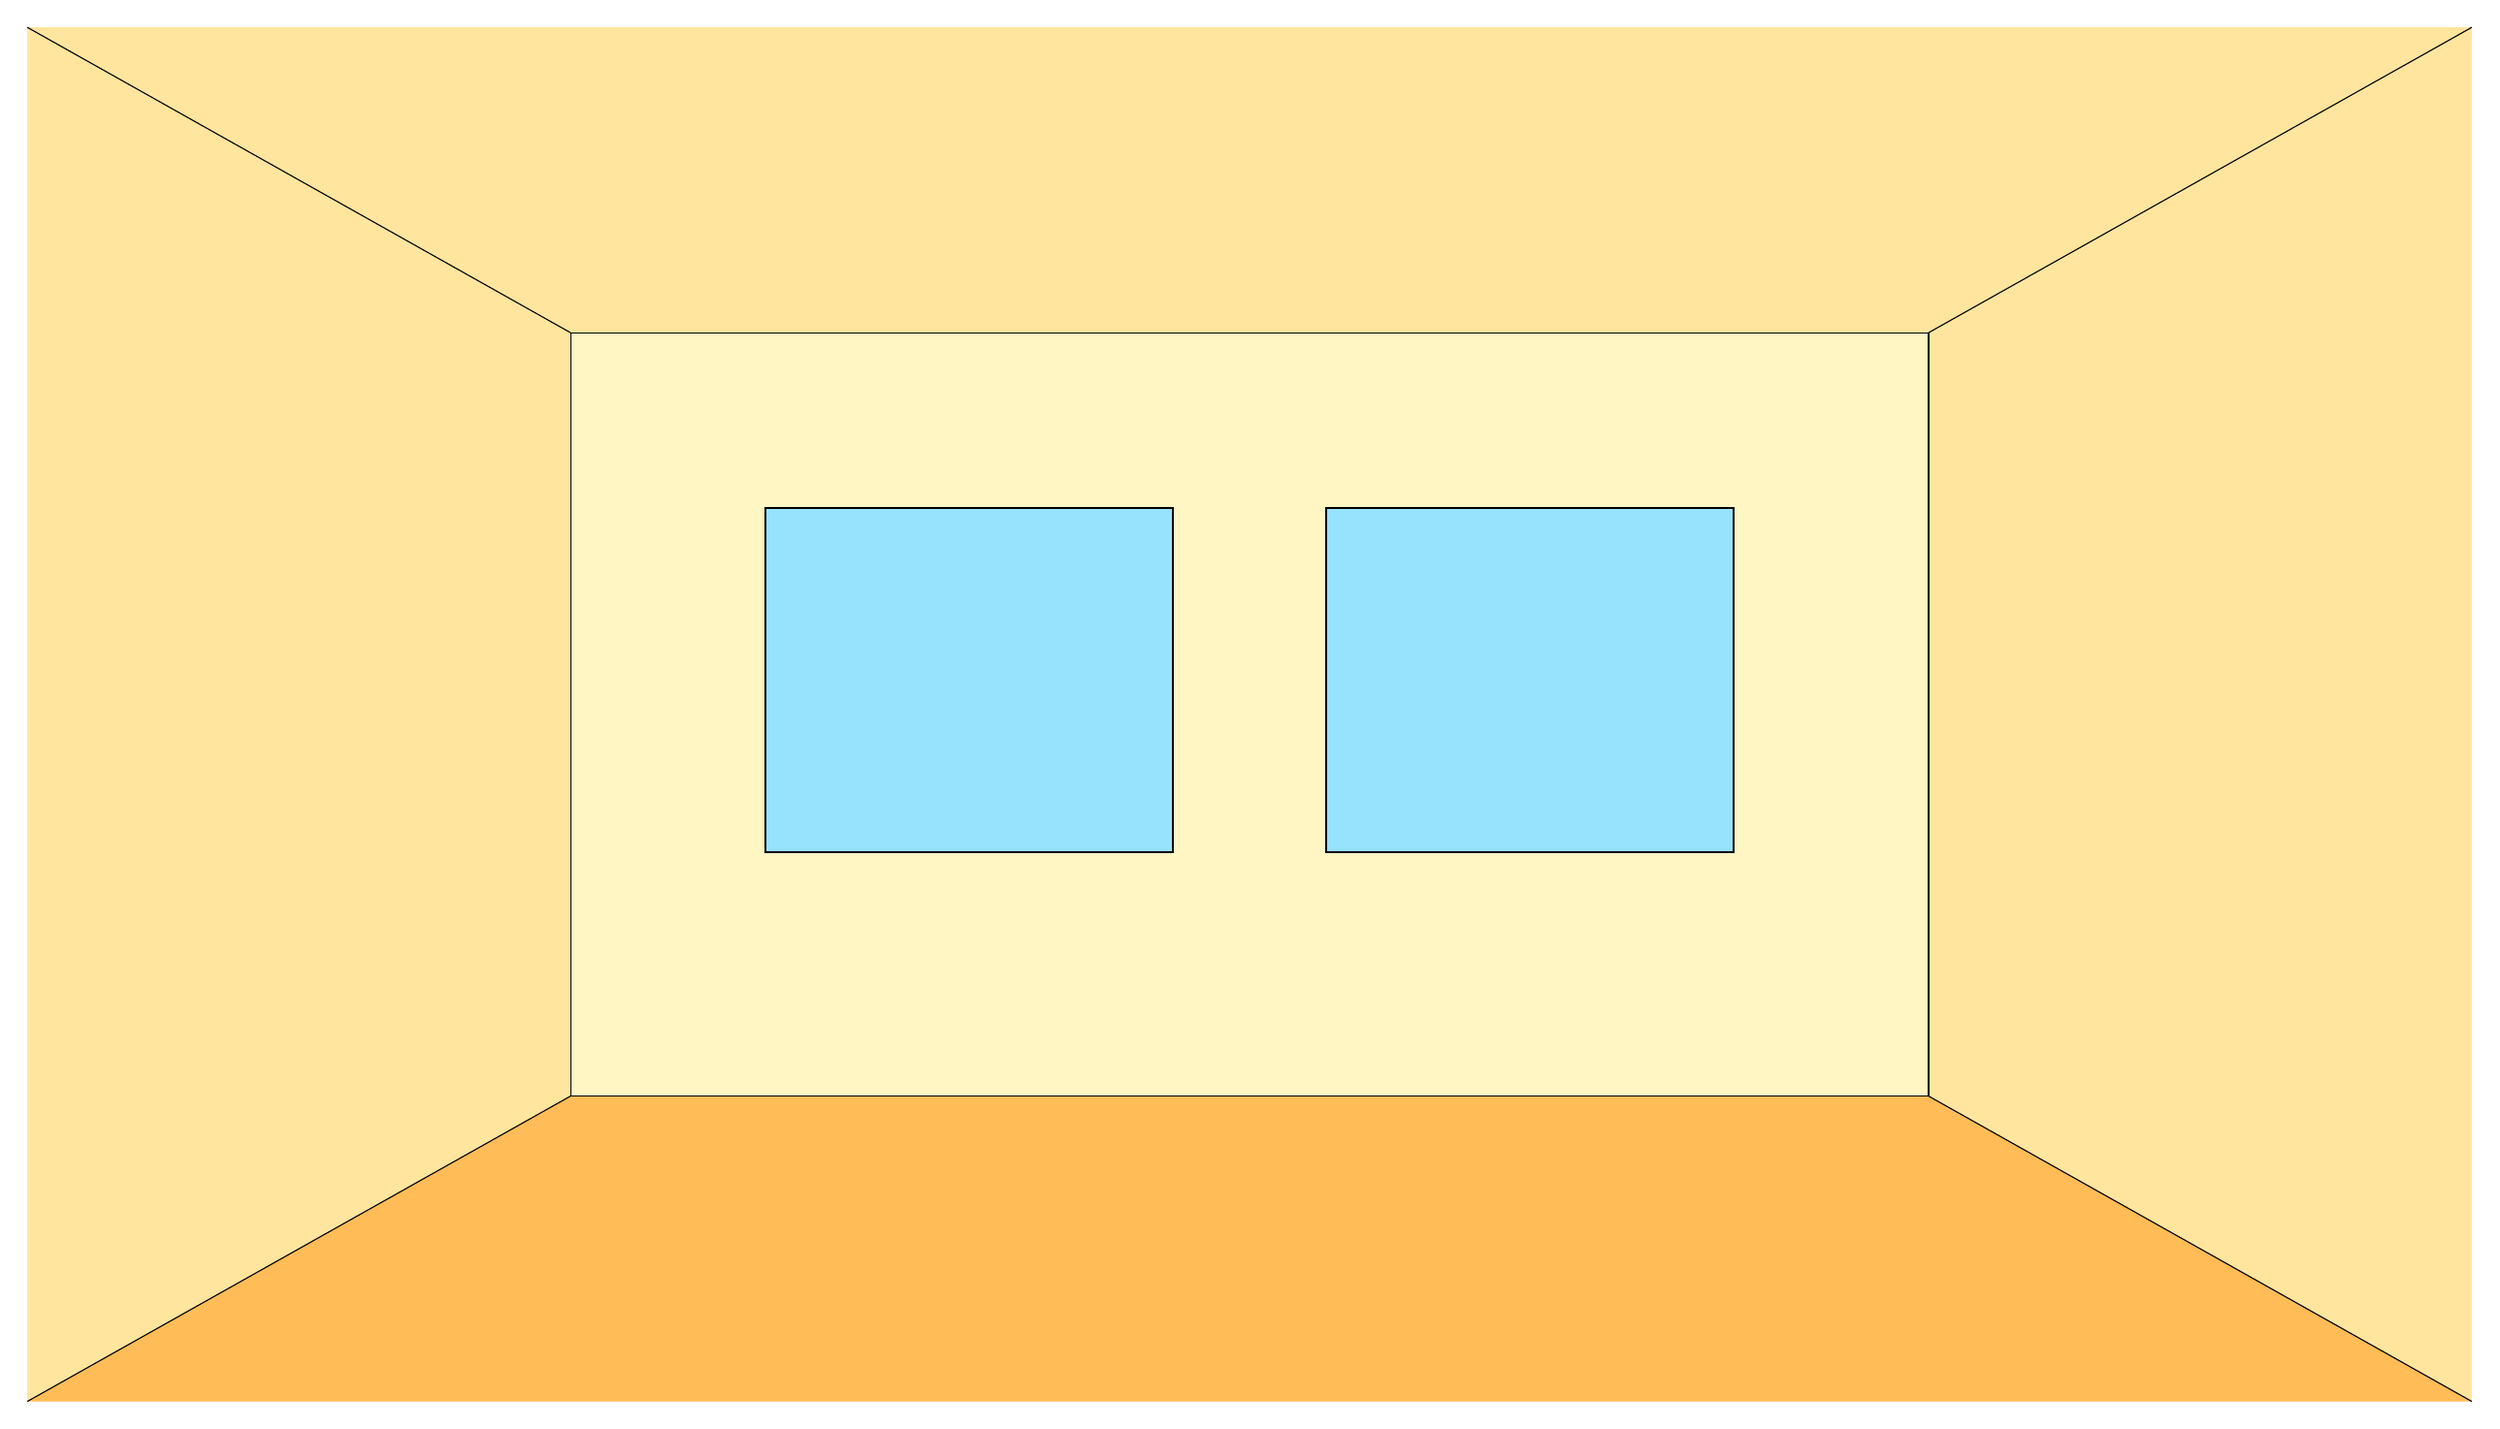
\begin{tikzpicture}[%
        % nodes size scales with picture
        % every node/.style={transform shape},
        % size
        % scale=0.7,
        % x=1cm,y=1cm
        ]
        
        \def\Lx{16};
        \def\Ly{9};
        \def\sff{1.8};  % front to back scale factor
        \coordinate (BLf) at (-\Lx,-\Ly);  % bottom left front corner
        \coordinate (BRf) at (\Lx,-\Ly);  % bottom right front corner
        \coordinate (TRf) at (\Lx,\Ly);  % top left front corner
        \coordinate (TLf) at (-\Lx,\Ly);  % top right front corner
        \coordinate (BLb) at (-\Lx/\sff,-\Ly/\sff);  % bottom left back corner
        \coordinate (BRb) at (\Lx/\sff,-\Ly/\sff);  % bottom right back corner
        \coordinate (TRb) at (\Lx/\sff,\Ly/\sff);  % top left back corner
        \coordinate (TLb) at (-\Lx/\sff,\Ly/\sff);  % top right back corner

        \definecolor{wallcolor}{RGB}{255, 229, 158}
        \definecolor{backcolor}{RGB}{255, 246, 196}
        \definecolor{floorcolor}{RGB}{255, 188, 87}
        \definecolor{skycolor}{RGB}{151, 226, 252}
        
        % paint walls and floor
        \fill[wallcolor] (BLf) -- (BLb) -- (TLb) -- (TRb) -- (BRb) -- (BRf) -- (TRf) -- (TLf);
        \fill[backcolor] (BLb) rectangle (TRb);
        \fill[floorcolor] (BLf) -- (BLb) -- (BRb) -- (BRf);

        % draw room edges
        % \draw (BLf) rectangle (TRf);
        \draw (BLb) rectangle (TRb);
        \draw (BLf) -- (BLb);
        \draw (BRf) -- (BRb);
        \draw (TLf) -- (TLb);
        \draw (TRf) -- (TRb);

        % draw back wall
        \begin{scope}[shift={(0,0)}]
            % draw windows
            \draw[thick,fill=skycolor] (-\Lx/16,-\Ly/5) rectangle ++(-\Lx/3.,\Ly/2);
            \draw[thick,fill=skycolor] (\Lx/16,-\Ly/5) rectangle ++(\Lx/3.,\Ly/2);
        \end{scope}


    \end{tikzpicture}
\end{document}a